\subsection{Naive beginnings}
\label{sec:naive_beginnigs}
We start by modelling the states of the agents:

\begin{HaskellCode}
data SIRState = Susceptible | Infected TimeDelta | Recovered
\end{HaskellCode}

Agents are ill for some duration, meaning we need to keep track when a potentially infected agent recovers. Also a simulation is stepped in discrete or continuous time-steps thus we introduce a notion of \textit{time} and $\Delta t$ by defining:

\begin{HaskellCode}
type Time      = Double
type TimeDelta = Double
\end{HaskellCode}

Now we can represent every agent simply as the SIR state which includes its potential recovery time. We hold all our agents in a list:
\begin{HaskellCode}
type SIRAgent = SIRState
type Agents   = [SIRAgent]
\end{HaskellCode}

Next we need to think about how to actually step our simulation. For this we define a function which advances our simulation with a fixed $\Delta t$ until a given time $t$ where in each step the agents are processed and the output is fed back into the next step. This is the source of pro-activity as agents are executed in every time step and can thus initiate actions based on the passing of time.
As already mentioned, the agent-based implementation of the SIR model is inherently stochastic which means we need access to a random-number generator. We decided to use the Random Monad at this point as threading a generator through the simulation and the agents could become very cumbersome. Thus our simulation stepping runs in the Random Monad:
TODO: make clear we are stepping by a dt of 1.0 which is necessary below

\begin{HaskellCode}
runSimulation :: RandomGen g 
  => Time -> Agents -> Rand g [Agents]
runSimulation tEnd as = runSimulationAux 0 as []
  where
    runSimulationAux :: RandomGen g 
      => Time -> Agents -> [Agents] -> Rand g [Agents]
    runSimulationAux t as acc
      | t >= tEnd = return (reverse (as : acc))
      | otherwise = do
        as' <- stepSimulation as 
        runSimulationAux (t + 1.0) as' (as : acc)

stepSimulation :: RandomGen g => Agents -> Rand g Agents
stepSimulation as = mapM (runAgent as) as
\end{HaskellCode}

Now we can implement the behaviour of an individual agent. First we need to distinguish between the agents SIR states:

\begin{HaskellCode}
processAgent :: RandomGen g 
  => Agents -> SIRAgent -> Rand g SIRAgent
processAgent as Susceptible    = susceptibleAgent as
processAgent _  (Infected dur) = return (infectedAgent dur)
processAgent _  Recovered      = return Recovered
\end{HaskellCode}

An agent gets fed the states of all agents in the system from the previous time-step so it can draw random contacts - this is one, very naive way of implementing the interactions between agents.

From our implementation it becomes apparent that only the behaviour of a susceptible agent involves randomness and that a recovered agent is simply a sink - it does nothing and stays constant.

Lets look how we can implement the behaviour of a susceptible agent. It simply makes contact on average with a number of other agents and gets infected with a given probability if an agent it has contact with is infected.
When the agent gets infected, it calculates also its time of recovery by drawing a random number from the exponential distribution, meaning it is ill on average for \textit{illnessDuration}.
TODO: make clear that this only works for dt=1.0, if we change dt then we would need to adjust contact rate (multiply) but the discretisation using floor will lead to wrong results

\begin{HaskellCode}
susceptibleAgent :: RandomGen g => Agents -> Rand g SIRAgent
susceptibleAgent as = do
    -- draws from exponential distribution
    rc <- randomExpM (1 / contactRate) 
    cs <- replicateM (floor rc) (makeContact as)
    if or cs
      then infect
      else return Susceptible
  where
    makeContact :: RandomGen g => Agents -> Rand g Bool
    makeContact as = do
      randContact <- randomElem as
      case randContact of
        -- returns True with given probability 
        (Infected _) -> randomBoolM infectivity 
        _            -> return False

    infect :: RandomGen g => Rand g SIRAgent
    infect = randomExpM (1 / illnessDuration) 
               >>= \rd -> return (Infected rd)
\end{HaskellCode}

The infected agent is trivial. It simply recovers after the given illness duration which is implemented as follows:
TODO: explain that we are using fixed dt=1.0

\begin{HaskellCode}
infectedAgent :: TimeDelta -> TimeDelta -> SIRAgent
infectedAgent dur
    | dur' <= 0 = Recovered
    | otherwise = Infected dur'
  where
    dur' = dur - 1.0  
\end{HaskellCode}

\subsubsection{Results}
When running our naive implementation with a population size of 1,000 we get the dynamics as seen in Figure \ref{fig:sir_abs_dynamics_naive}. When comparing it to the dynamics of the analytical solution in Figure \ref{fig:sir_sd_dynamics}, the agent-based dynamics are not as smooth which stems from the fact that the agent-based approach is inherently discrete and stochastic \cite{macal_agent-based_2010}. Also we are using a $\Delta t = 1.0$ which means that we are under-sampling the contact-rate. We will will address this problem in the next section.

\begin{figure}
	\centering
	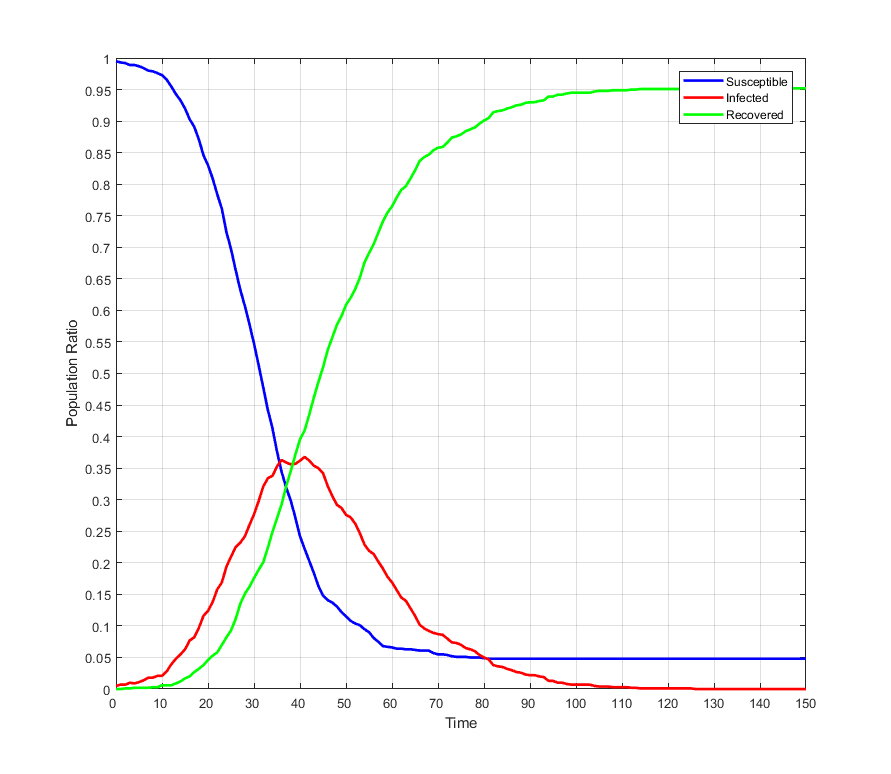
\includegraphics[width=0.35\textwidth, angle=0]{./fig/step1_randmonad/SIR_1000agents_150t_1dt.png}
	\caption{Naive simulation of SIR using the agent-based approach. Population of 1,000, contact rate $\beta = \frac{1}{5}$, infection probability $\gamma = 0.05$, illness duration $\delta = 15$ with initially 1 infected agent. Simulation run for 150 time-steps with fixed $\Delta t = 1.0$.}
	\label{fig:sir_abs_dynamics_naive}
\end{figure}

%\begin{figure}
%\begin{center}
%	\begin{tabular}{c}
%		\begin{subfigure}[b]{0.2\textwidth}
%			\centering
%			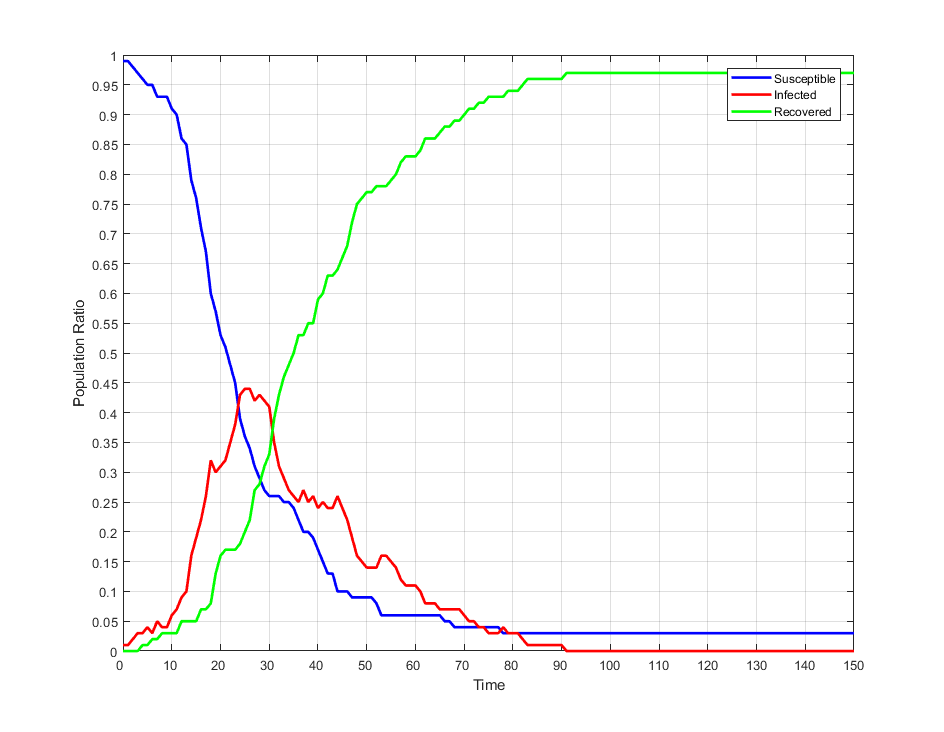
\includegraphics[width=1.0\textwidth, angle=0]{./fig/step1_randmonad/SIR_100agents_150t_1dt.png}
%			\caption{100 Agents}
%			\label{fig:sir_abs_approximating_1dt_100agents}
%		\end{subfigure}
    	
%    	&
%    	
%		\begin{subfigure}[b]{0.30\textwidth}
%			\centering
%			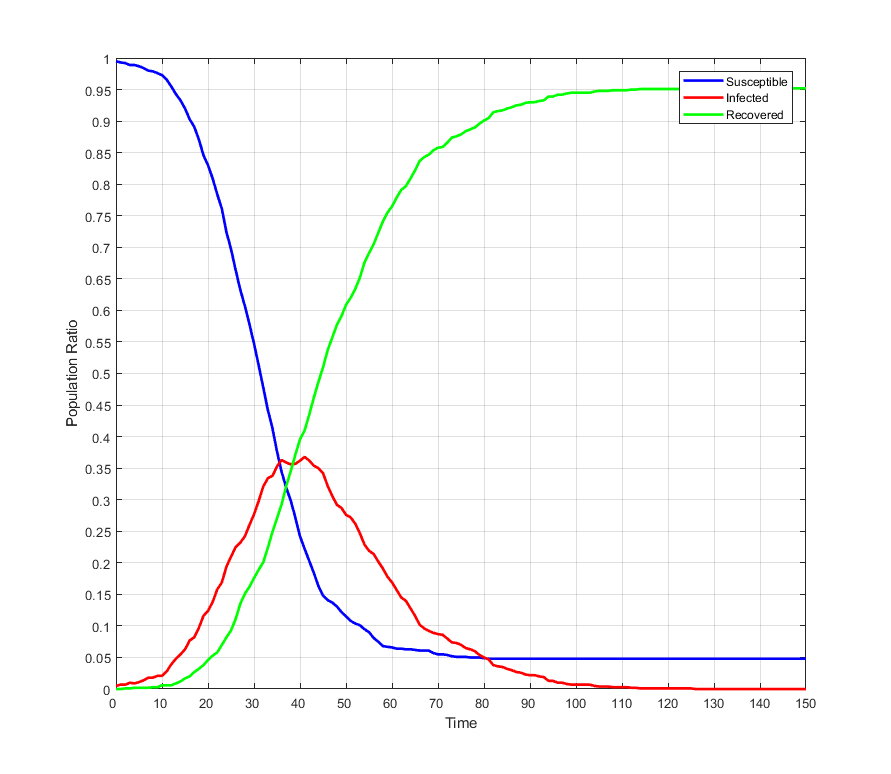
\includegraphics[width=1.0\textwidth, angle=0]{./fig/step1_randmonad/SIR_1000agents_150t_1dt.png}
%			\caption{1,000 Agents}
%			\label{fig:sir_abs_approximating_1dt_1000agents}
%		\end{subfigure}
%	\end{tabular}
%	\caption{TODO: use only 1000, a simulation with 100 has slightly different dynamics in SD as well! Naive simulation of SIR using the agent-based approach. Varying population size, contact rate $\beta = \frac{1}{5}$, infection probability $\gamma = 0.05$, illness duration $\delta = 15$ with initially 1 infected agent. Simulation run for 150 time-steps with fixed $\Delta t = 1.0$.} 
%	\label{fig:sir_abs_dynamics_naive}
%\end{center}
%\end{figure}

\subsubsection{Discussion}
Reflecting on our first naive approach we can conclude that it already introduced most of the fundamental concepts of ABS
\begin{itemize}
	\item Time - the simulation occurs over virtual time which is modelled explicitly divided into \textit{fixed} $\Delta t$ where at each step all agents are executed.
	\item Agents - we implement each agent as an individual, with the behaviour depending on its state.
	\item Feedback - the output state of the agent in the current time-step $t$ is the input state for the next time-step $t + \Delta t$.
	\item Environment - as environment we implicitly assume a fully-connected network (complete graph) where every agent 'knows' every other agent, including itself and thus can make contact with all of them.
	\item Stochasticity - it is an inherently stochastic simulation, which is indicated by the Random Monad type and the usage of \textit{randomBoolM} and \textit{randomExpM}.
	\item Deterministic - repeated runs with the same initial random-number generator result in same dynamics. This may not come as a surprise but in Haskell we can guarantee that property statically already at compile time because our simulation runs in the Random Monad and \textit{not} in the IO Monad. This guarantees that no external, uncontrollable sources of randomness can interfere with the simulation.
	\item Dynamics - with increasing number of agents the dynamics smooth out \cite{macal_agent-based_2010}.
\end{itemize}

TODO: problem is that we implicitly assume that TimeDelta is always 1.0, still it is not ensured in all agents

Nonetheless our approach has also weaknesses and dangers:
\begin{enumerate}
	\item We are implicitly assuming that our implementation is sampling with 1.0
	\item $\Delta t$ is passed explicitly as argument to the agent and needs to be dealt with explicitly. This is not very elegant and a potential source of errors - can we do better and find a more elegant solution? 
	\item The way our agents are represented is not very modular. The state of the agent is explicitly encoded in an ADT and when processing the agent, the behavioural function always needs to distinguish between the states. Can we express it in a more modular way e.g. continuations?
\end{enumerate}

We now move on to the next section in which we will address these points and the under-sampling issue.